\begin{figure}[t]
    \centering
    \FloatBarrier
    \sidecaption{Conceptual model of the learning paradigms, wherein the number of unlabeled source images and labeled and unlabeled target images serve
as the axes. Not having target labels is common, as it otherwise becomes either semi-supervised or supervised learning. Two scenarios only differ in the number of target images (source-free and test-time domain adaptation [SFDA and TTDA, respectively]) and one has no target images available (self-supervised learning).\label{fig:da_cube}
}
    \resizebox{\columnwidth}{!}{%



\tikzset{every picture/.style={line width=0.75pt}} %set default line width to 0.75pt        

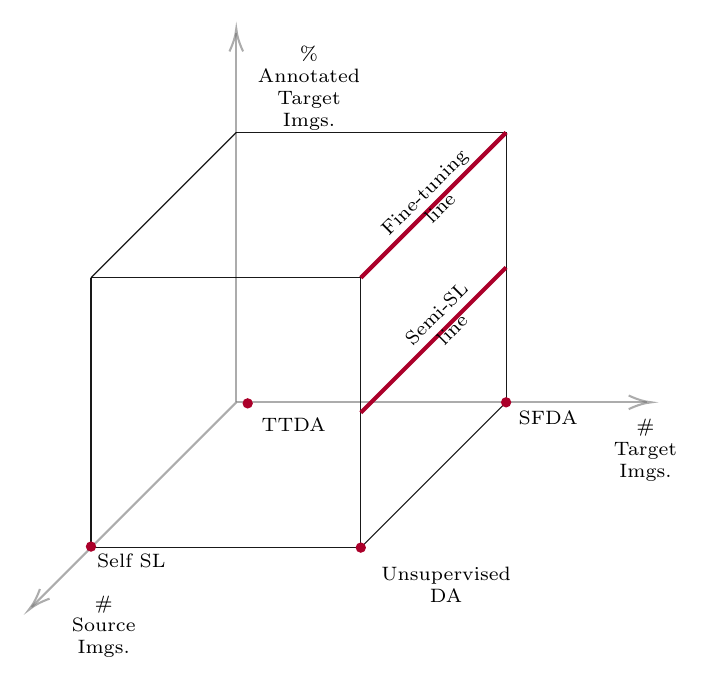
\begin{tikzpicture}[x=0.75pt,y=0.75pt,yscale=-1,xscale=1]
%uncomment if require: \path (0,402); %set diagram left start at 0, and has height of 402

%Straight Lines [id:da6807006831993536] 
\draw [color={rgb, 255:red, 117; green, 117; blue, 117 }  ,draw opacity=0.6 ][line width=0.75]    (270,210) -- (270,32) ;
\draw [shift={(270,30)}, rotate = 90] [color={rgb, 255:red, 117; green, 117; blue, 117 }  ,draw opacity=0.6 ][line width=0.75]    (10.93,-3.29) .. controls (6.95,-1.4) and (3.31,-0.3) .. (0,0) .. controls (3.31,0.3) and (6.95,1.4) .. (10.93,3.29)   ;
%Straight Lines [id:da5295149315723777] 
\draw [color={rgb, 255:red, 117; green, 117; blue, 117 }  ,draw opacity=0.6 ][line width=0.75]    (270,210) -- (468,210) ;
\draw [shift={(470,210)}, rotate = 180] [color={rgb, 255:red, 117; green, 117; blue, 117 }  ,draw opacity=0.6 ][line width=0.75]    (10.93,-3.29) .. controls (6.95,-1.4) and (3.31,-0.3) .. (0,0) .. controls (3.31,0.3) and (6.95,1.4) .. (10.93,3.29)   ;
%Straight Lines [id:da534666056608414] 
\draw [color={rgb, 255:red, 117; green, 117; blue, 117 }  ,draw opacity=0.6 ][line width=0.75]    (270,210) -- (171.41,308.59) ;
\draw [shift={(170,310)}, rotate = 315] [color={rgb, 255:red, 117; green, 117; blue, 117 }  ,draw opacity=0.6 ][line width=0.75]    (10.93,-3.29) .. controls (6.95,-1.4) and (3.31,-0.3) .. (0,0) .. controls (3.31,0.3) and (6.95,1.4) .. (10.93,3.29)   ;
%Straight Lines [id:da0025027309814475984] 
\draw [color={rgb, 255:red, 0; green, 0; blue, 0 }  ,draw opacity=0.9 ]   (270,80) -- (400,80) ;
%Straight Lines [id:da3170933147390458] 
\draw [color={rgb, 255:red, 0; green, 0; blue, 0 }  ,draw opacity=0.9 ]   (400,80) -- (400,210) ;
%Straight Lines [id:da8084774068453204] 
\draw [color={rgb, 255:red, 0; green, 0; blue, 0 }  ,draw opacity=0.9 ]   (400,210) -- (330,280) ;
%Straight Lines [id:da14868444296828032] 
\draw [color={rgb, 255:red, 0; green, 0; blue, 0 }  ,draw opacity=0.9 ]   (200,280) -- (330,280) ;
%Straight Lines [id:da9908929804494571] 
\draw [color={rgb, 255:red, 0; green, 0; blue, 0 }  ,draw opacity=0.9 ]   (330,150) -- (330,280) ;
%Straight Lines [id:da0019316496763430724] 
\draw [color={rgb, 255:red, 0; green, 0; blue, 0 }  ,draw opacity=0.9 ]   (200,150) -- (200,280) ;
%Straight Lines [id:da7518926340375516] 
\draw [color={rgb, 255:red, 0; green, 0; blue, 0 }  ,draw opacity=0.9 ]   (200,150) -- (330,150) ;
%Straight Lines [id:da3769124480681334] 
\draw [color={rgb, 255:red, 0; green, 0; blue, 0 }  ,draw opacity=0.9 ]   (270,80) -- (200,150) ;
%Straight Lines [id:da5228594606876449] 
\draw [color={rgb, 255:red, 171; green, 0; blue, 42 }  ,draw opacity=1 ][line width=1.5]    (400,145) -- (330,215) ;
%Straight Lines [id:da4767901038712239] 
\draw [color={rgb, 255:red, 171; green, 0; blue, 42 }  ,draw opacity=1 ][line width=1.5]    (400,80) -- (330,150) ;
%Shape: Circle [id:dp5300687249748464] 
\draw  [draw opacity=0][fill={rgb, 255:red, 171; green, 0; blue, 42 }  ,fill opacity=1 ] (327.5,280) .. controls (327.5,278.62) and (328.62,277.5) .. (330,277.5) .. controls (331.38,277.5) and (332.5,278.62) .. (332.5,280) .. controls (332.5,281.38) and (331.38,282.5) .. (330,282.5) .. controls (328.62,282.5) and (327.5,281.38) .. (327.5,280) -- cycle ;
%Shape: Circle [id:dp9711792189769151] 
\draw  [draw opacity=0][fill={rgb, 255:red, 171; green, 0; blue, 42 }  ,fill opacity=1 ] (273,210.5) .. controls (273,209.12) and (274.12,208) .. (275.5,208) .. controls (276.88,208) and (278,209.12) .. (278,210.5) .. controls (278,211.88) and (276.88,213) .. (275.5,213) .. controls (274.12,213) and (273,211.88) .. (273,210.5) -- cycle ;
%Shape: Circle [id:dp6127433690927064] 
\draw  [draw opacity=0][fill={rgb, 255:red, 171; green, 0; blue, 42 }  ,fill opacity=1 ] (397.5,210) .. controls (397.5,208.62) and (398.62,207.5) .. (400,207.5) .. controls (401.38,207.5) and (402.5,208.62) .. (402.5,210) .. controls (402.5,211.38) and (401.38,212.5) .. (400,212.5) .. controls (398.62,212.5) and (397.5,211.38) .. (397.5,210) -- cycle ;
%Shape: Circle [id:dp8193525877009633] 
\draw  [draw opacity=0][fill={rgb, 255:red, 171; green, 0; blue, 42 }  ,fill opacity=1 ] (197.5,279.5) .. controls (197.5,278.12) and (198.62,277) .. (200,277) .. controls (201.38,277) and (202.5,278.12) .. (202.5,279.5) .. controls (202.5,280.88) and (201.38,282) .. (200,282) .. controls (198.62,282) and (197.5,280.88) .. (197.5,279.5) -- cycle ;

% Text Node
\draw (275,37) node [anchor=north west][inner sep=0.75pt]  [font=\scriptsize] [align=left] {\begin{minipage}[lt]{43.21pt}\setlength\topsep{0pt}
\begin{center}
\% Annotated\\Target Imgs.
\end{center}

\end{minipage}};
% Text Node
\draw (447,217) node [anchor=north west][inner sep=0.75pt]  [font=\scriptsize] [align=left] {\begin{minipage}[lt]{28.38pt}\setlength\topsep{0pt}
\begin{center}
\# Target\\Imgs.
\end{center}

\end{minipage}};
% Text Node
\draw (184,302) node [anchor=north west][inner sep=0.75pt]  [font=\scriptsize] [align=left] {\begin{minipage}[lt]{31.29pt}\setlength\topsep{0pt}
\begin{center}
\# Source\\Imgs.
\end{center}

\end{minipage}};
% Text Node
\draw (331,288) node [anchor=north west][inner sep=0.75pt]  [font=\scriptsize] [align=left] {\begin{minipage}[lt]{58.26pt}\setlength\topsep{0pt}
\begin{center}
Unsupervised DA
\end{center}

\end{minipage}};
% Text Node
\draw (404.5,213) node [anchor=north west][inner sep=0.75pt]  [font=\scriptsize] [align=left] {\begin{minipage}[lt]{21.76pt}\setlength\topsep{0pt}
\begin{center}
SFDA
\end{center}

\end{minipage}};
% Text Node
\draw (342.12,185.25) node [anchor=north west][inner sep=0.75pt]  [font=\scriptsize,rotate=-315] [align=left] {\begin{minipage}[lt]{42.92pt}\setlength\topsep{0pt}
\begin{center}
Semi-SL line
\end{center}

\end{minipage}};
% Text Node
\draw (332.12,130.81) node [anchor=north west][inner sep=0.75pt]  [font=\scriptsize,rotate=-315] [align=left] {\begin{minipage}[lt]{51.53pt}\setlength\topsep{0pt}
\begin{center}
Fine-tuning line
\end{center}

\end{minipage}};
% Text Node
\draw (281,212) node [anchor=north west][inner sep=0.75pt]  [font=\scriptsize] [align=left] {\begin{minipage}[lt]{21.36pt}\setlength\topsep{0pt}
\begin{center}
TTDA
\end{center}

\end{minipage}};
% Text Node
\draw (201,282) node [anchor=north west][inner sep=0.75pt]  [font=\scriptsize] [align=left] {\begin{minipage}[lt]{25.74pt}\setlength\topsep{0pt}
\begin{center}
Self SL
\end{center}

\end{minipage}};


\end{tikzpicture}
}
\end{figure}